% TEMPLATE for Usenix papers, specifically to meet requirements of
%  USENIX '05
% originally a template for producing IEEE-format articles using LaTeX.
%   written by Matthew Ward, CS Department, Worcester Polytechnic Institute.
% adapted by David Beazley for his excellent SWIG paper in Proceedings,
%   Tcl 96
% turned into a smartass generic template by De Clarke, with thanks to
%   both the above pioneers
% use at your own risk.  Complaints to /dev/null.
% make it two column with no page numbering, default is 10 point

% Munged by Fred Douglis <douglis@research.att.com> 10/97 to separate
% the .sty file from the LaTeX source template, so that people can
% more easily include the .sty file into an existing document.  Also
% changed to more closely follow the style guidelines as represented
% by the Word sample file. 

% Note that since 2010, USENIX does not require endnotes. If you want
% foot of page notes, don't include the endnotes package in the 
% usepackage command, below.

\documentclass[letterpaper,twocolumn,10pt]{article}
\usepackage{usenix,epsfig,endnotes,parskip,amsmath,amssymb,stfloats,placeins}
\begin{document}

%don't want date printed
\date{}

%make title bold and 14 pt font (Latex default is non-bold, 16 pt)
\title{\Large \bf A Protocol for Interledger Payments}

\author{
\textnormal{Stefan Thomas \& Evan Schwartz} \\
\textnormal{\texttt{\{stefan,evan\}@ripple.com}}
}

\maketitle

% Use the following at camera-ready time to suppress page numbers.
% Comment it out when you first submit the paper for review.
\thispagestyle{empty}

\section*{Abstract}

A protocol for payments across payment systems would enable payments to be made from any sender to any recipient even if they do not share a common payment system or \textit{ledger}. We introduce a protocol for interledger payments using escrowed transfers. It removes the need for the sender and recipient to trust the \textit{connectors} facilitating payments between their ledgers. Anyone can create new connections between ledgers and compete to provide the fastest, lowest cost payments. This creates a more accessible, competitive and resilient global financial system.

\section{Introduction}

% TODO talk more about scalability

Sending money today within any single payment system or \textit{ledger} is relatively simple, fast and inexpensive. However, moving money between systems is cumbersome, slow and costly, if it is possible at all. There are few connections between payment systems because intermediaries must be highly trusted counterparties that can be relied upon not to fail or disappear with the sender's money.

We present a protocol for \mbox{\textit{interledger}} payments that removes the need for the sender and recipient to trust the \textit{connectors} facilitating payments between their ledgers. It uses ledger-provided escrow to guarantee the sender of a payment will either have a non-repudiable receipt confirming that the recipient has been paid, or their escrowed funds will be returned. The protocol does not rely on any global ledger, centralized or decentralized, for processing payments. It enables anyone to create new connections between ledgers of all types by removing the trust from interledger connectors. This allows all payments to take advantage of a highly competitive market for the best rates and speed.

The protocol enables payments to be chained, giving all payment systems equal global reach. This makes every item of value spendable anywhere---from fiat or cryptocurrencies, to commodities, loyalty points, computing resources and social credit.

The protocol has two modes for executing payments: \textit{universal} and \textit{atomic}.
% which enable participants to optimize between...

The \textit{universal} mode guarantees the sender a cryptographically signed receipt from the recipient or the return of their escrowed funds, even when the sender, recipient and connectors do not share trust in any institution or system. This mode provides safety and liveness for non-faulty participants connected to non-faulty ledgers under a strict synchrony assumption. Even when synchrony is violated (i.e. messages are delayed longer than expected), safety is maintained from the sender's perspective. In this case, connectors bear a risk of losing escrowed funds, which they can account for in their fees.

% TODO ^ Haven't defined participants.

The \textit{atomic} mode removes the messaging delay risks to connectors for payments in which the participants can agree upon a group of \textit{notaries} to determine the outcome of the payment. Notaries use a Byzantine fault-tolerant binary agreement protocol to provide safety and liveness provided at most $f$ out of a total of $3f + 1$ notaries are simultaneously faulty.

% The \textit{atomic} mode provides atomicity and tolerates arbitrary or malicious behavior using a Byzantine fault-tolerant binary agreement protocol. This reduces the risks connectors incur for payments in which the sender, recipient and connectors can agree upon a group of \mbox{\textit{notaries}}.

This protocol provides:
\begin{itemize}
\item A guarantee for a payment's sender of a cryptographically signed receipt from the recipient or a return of their escrowed funds.
\item Chained payments through arbitrary sequences of ledgers and untrusted connectors.
\item Two modes of payment execution that provide safety and liveness under assumptions of strong or eventual synchrony, depending on participants' level of shared trust.
\end{itemize}

% We present a protocol for interledger payments through chains of ledgers and untrusted connectors. It uses ledger-provided escrow to guarantee the sender of a payment will either have non-repudiable proof that the recipient has been paid or their escrowed funds will be returned. 

% The protocol has two modes: \textit{universal} and \textit{atomic}.

% The universal mode enables payments across an arbitrary chain of connectors that do not all share trust in any institution or system. They must only agree on a cryptographic signature scheme for the common execution condition. The sender and recipient are isolated from the risk of any failures of a connector or intermediary ledger. The connectors assume only the risks associated with the failure of a ledger they trust directly, and price these risks into their fees.

% The atomic mode provides full atomicity---certainty that payments cannot partially execute, which protects the connectors from risk---for a payment chain in which the sender, recipient and connectors can agree upon a notary or group of notaries.

% OLD

% What is needed is a protocol for \mbox{\textit{interledger}} payments that removes the need for the sender and recipient to trust the \textit{connectors} facilitating payments between their ledgers. Removing the trust in the intermediaries enables anyone to create new connections between ledgers and allows individuals and institutions to take advantage of a highly competitive market for the best rates and speed for every payment.

% % TODO mention that it doesn't depend on any one ledger, centralized or decentralized

% Such a protocol further enables payments to be chained, giving all payment systems equal global reach. This makes every item of value spendable anywhere, from fiat or cryptocurrencies, to commodities, loyalty points, computing resources and social credit.

% Reducing the barriers to creating new connections between a multitude of ledgers creates a more accessible, competitive and resilient global financial system.

% We present a protocol for interledger payments through chains of ledgers and untrusted connectors. It uses ledger-provided escrow to guarantee the sender of a payment will either have non-repudiable proof that the recipient has been paid or their escrowed funds will be returned. 

% The protocol has two modes: \textit{universal} and \textit{atomic}.

% The universal mode enables payments across an arbitrary chain of connectors that do not all share trust in any institution or system. They must only agree on a cryptographic signature scheme for the common execution condition. The sender and recipient are isolated from the risk of any failures of a connector or intermediary ledger. The connectors assume only the risks associated with the failure of a ledger they trust directly, and price these risks into their fees.

% The atomic mode provides full atomicity---certainty that payments cannot partially execute, which protects the connectors from risk---for a payment chain in which the sender, recipient and connectors can agree upon a notary or group of notaries.


\section{A Model of Interledger Payments}
% Alternatively: Generalized Interledger Payments

For interledger payments, we use a simple model consisting of \textit{ledgers} and \textit{connectors}.
                 
\subsection{Ledgers}

% TODO: note that the only criteria for being a ledger in this system is to track have transferable assets and to enforce cryptographic escrow

% TODO: note that a ledger can track anything of value, whether it's money or property or digital titles

Any digital payment system must enable payments between users while preventing double spending. Transfers between users or accounts are recorded in a \textit{ledger}, which may be centralized or decentralized. \cite{Bitcoin}

Figure \ref{fig:three-bells} shows an example book transfer from a sender Alice to a recipient Bob on a ledger where they both hold accounts.

\begin{figure}[ht]
    \centering
    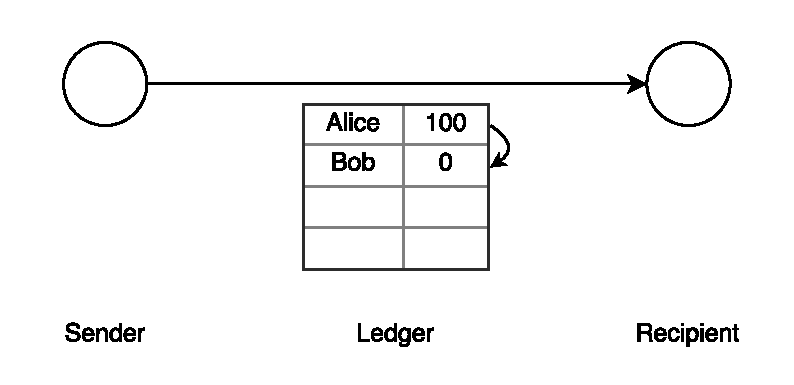
\includegraphics[width=\columnwidth]{figures/three-bells.pdf}
    \caption{Book transfer}
    \label{fig:three-bells}
\end{figure}

For the purposes of this model we consider a ledger to be a system for tracking a single type of asset. It may track ownership of divisible assets such as currency or shares, or non-divisible assets such as titles. If a payment system supports multiple assets, it is seen as maintaining multiple ledgers.

Individuals and institutions select the ledgers they use based upon diverse sets of preferences and use cases. Every ledger offers different characteristics in terms of enforcement of property rights, transferability, deposit and withdrawal, chargebacks, fees and other policies. It is not practical to expect one set of characteristics to support all use cases \cite{back2014enabling}, therefore we believe that what is most needed is a reliable, neutral way to connect diverse ledgers.

\subsection{Connectors}

A \textit{connector} is a system that facilitates interledger payments by coordinating transfers between multiple ledgers and, if necessary, translating between the different data formats of the ledgers. 

Connectors exchange a book transfer into their account on one ledger for a book transfer out of their account on another ledger. There are many possible arrangements that enable connectors to perform their function: they may be operated by the same entity as one of the ledgers or by third parties that have pre-funded accounts on both ledgers. All that matters from the outside, however, is that connectors are capable---for whatever reason---of facilitating interledger payments. Connectors earn the spread between the value of the two transfers as compensation for payment risk.

\begin{figure}[ht]
    \centering
    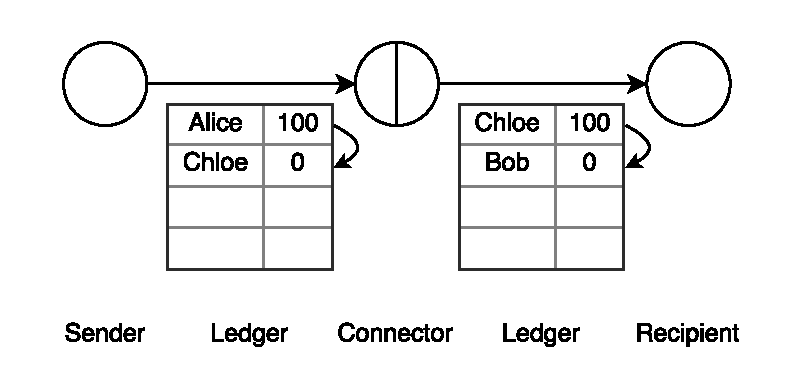
\includegraphics[width=\columnwidth]{figures/connector.pdf}
    \caption{Connector controls accounts on two ledgers}
    \label{fig:connector}
\end{figure}

More connectors can be added in parallel between ledgers to make their connection more robust and enable higher payment volume. Independently-operated and designed connectors especially increase the resiliency, as the failure of one is less likely to affect the others.

Even in cases where there is no direct connection between two ledgers, payments can be made between them if there is a \textit{chain of connectors} connecting them. Money is transferred from the origin ledger to an intermediary ledger through a connector and then onwards through a second connector, and so on through to the receiving ledger.
% TODO: Can we cite something that explains how these graph thingys get very easily very connected

As illustrated in Figure \ref{fig:parallel-path}, individual payments can take advantage of the liquidity and rates offered by multiple connectors simultaneously. The protocol works the same way whether it uses single or parallel paths. For simplicity, the examples throughout the rest of the paper will discuss payments with only one connector between each ledger and only one book transfer per ledger.

\begin{figure}[ht]
    \centering
    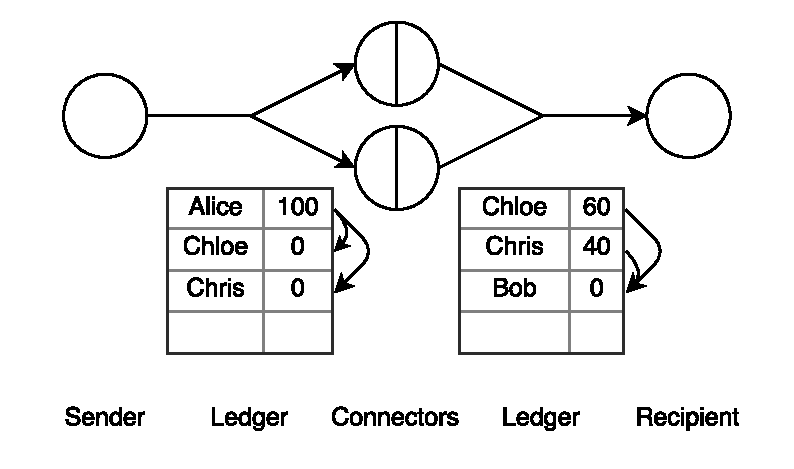
\includegraphics[width=\columnwidth]{figures/parallel-path.pdf}
    \caption{Connector controls accounts on two ledgers}
    \label{fig:parallel-path}
\end{figure}



%\subsection{Trust}

% TODO revise this section

%Each participant --- the sender, recipient, and connectors --- chooses which ledger or ledgers to hold accounts with. Every ledger offers different characteristics in terms of enforcement of property rights, transferability, deposit and withdrawal, chargebacks and other policies. Account holders accept the strengths and weaknesses of their ledger, but they should not be exposed to any risk from faulty or malicious behavior on the part of the other participants in an interledger payment.

% ES we may need to flesh this section out a little bit more to make it clear

% Even though the different account holders do not trust each other, ledgers and connectors can create links in a chain that extends all the way from the sender to the recipient.

%TODO graphic
%     |       |
% S ( | ) C ( | ) R
%     |       |

\section{Universal Interledger Payments}

\begin{figure*}[th!]
    \centering
    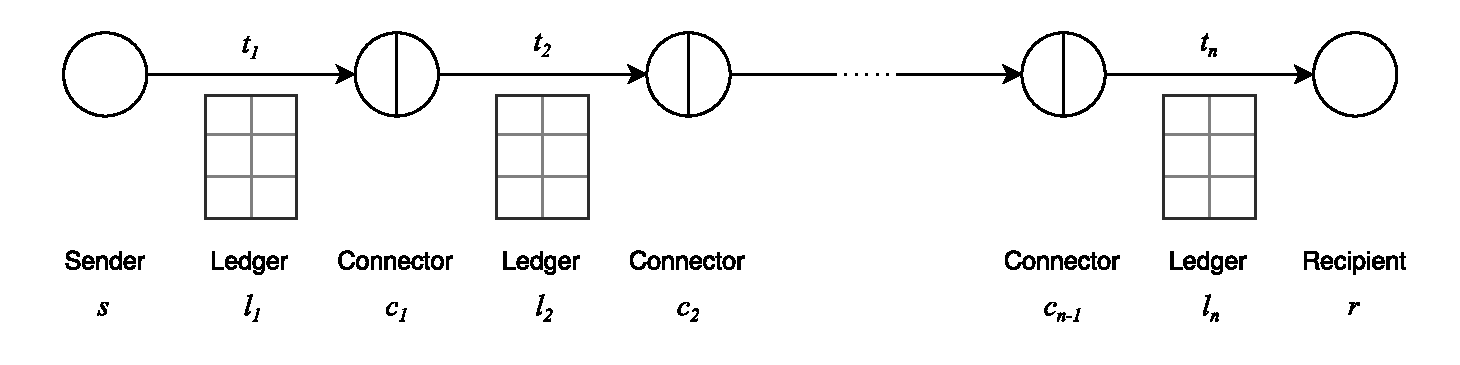
\includegraphics[width=\textwidth]{figures/payment-chain.pdf}
    \caption{Payment chain}
    \label{fig:n-bells}
\end{figure*}

The \textit{universal} mode of the interledger payment protocol uses cryptographic escrow and an ordering of transfers designed to eliminate payment risk for the sender and recipient, and to minimize risk for the connectors.

% TODO should we be more explicit and say that this is not fully atomic? or is that clear enough?

Funds are first placed in escrow by the sender and then the connectors on each of the ledgers in sequence from the sender to the recipient. The transfers are executed in reverse order, starting with the transfer to the recipient and going backwards down the chain, to ensure the connectors have strong incentives to see the payment execute correctly and completely.

Figure \ref{fig:n-bells} shows a payment from a sender $s$ to a recipient $r$. The payment consists of a set of $n$ book transfers $B$ on ledgers $L$, such that $ \left\vert{B}\right\vert = \left\vert{L}\right\vert = n $. The ledgers are connected by the set of $n-1$ connectors $C$, such that $ \left\vert{C}\right\vert = n-1 $. The sender $s$ has an account on ledger $l_1$ and the recipient $r$ has an account on ledger $l_n$. Each connector $c_i$ where $ \{ i \in \mathbb{Z}^+ : i < n \} $ has accounts on ledgers $l_i$ and $l_{i+1}$ and facilitates payments between them.



\subsection{Escrow}

Ledgers must support escrowed transfers to enable interledger payments for their account holders while isolating them from risk. Escrow protects the sender $s$ and assures the connectors in $C$ and the recipient $r$ that they will receive the funds once an execution condition $e$ is met. The participants must only trust the ledgers on which they hold accounts to properly enforce $e$, which isolates each participant from the risks of failure or malicious behavior elsewhere in the payment chain.

Figure \ref{fig:transfer-states} illustrates the possible states of a transfer, which mirror the states in a two-phase commit. \cite[p.~466]{Gray:1978:NDB:647433.723863}  When a transfer is first \textit{proposed}, the details of the transfer are shared with the participants, but no changes are made to the ledger. As soon as the affected account holders have authorized the transfer, the ledger checks that the funds are available and that all of its rules and policies have been satisfied. The ledger places the funds in escrow and the transfer is now \textit{prepared}. If the execution condition $e$ is met before the expiration time, the transfer is \textit{executed}. If any of the checks fail or the expiration time passes, the transfer is \textit{rejected} and the escrowed funds are returned to their originator.

\begin{figure}[ht]
    \centering
    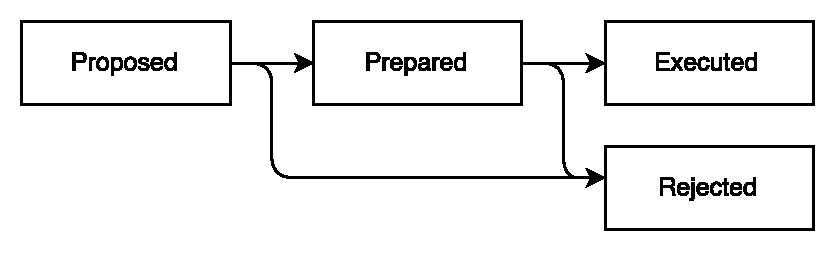
\includegraphics[width=\columnwidth]{figures/transfer-states.pdf}
    \caption{Transfer states}
    \label{fig:transfer-states}
\end{figure}

\begin{figure*}[h]
    \centering
    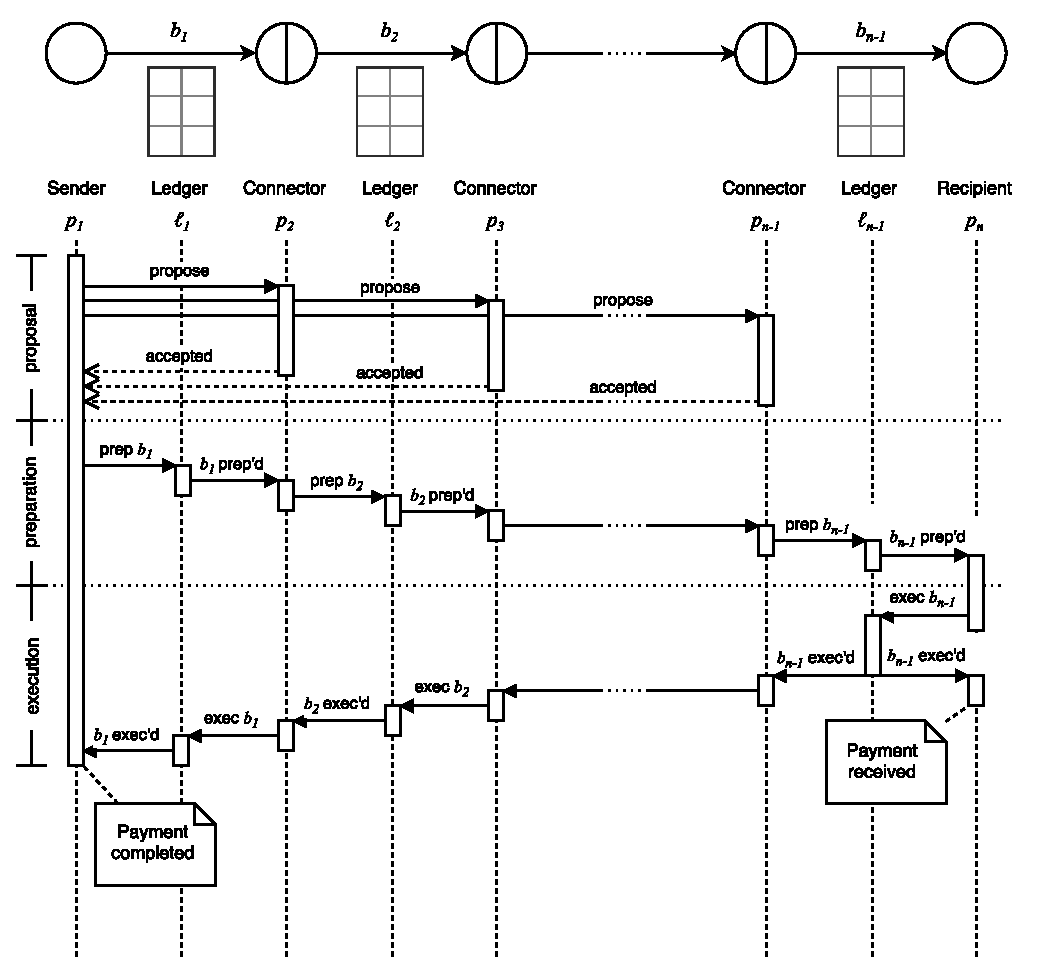
\includegraphics[width=\textwidth]{figures/universal-sequence.pdf}
    \caption{Phases of a payment in the universal mode}
    \label{fig:sequence}
\end{figure*}

\subsection{Execution Conditions}

Each book transfer $b_i \in B$ where 
% TODO should we say that n = |B| ?
$ \{ i \in \mathbb{Z}^+ : i \leq n \} $ is escrowed based on some execution condition $e_i$ describing events external to the ledger. A simple way to securely communicate the outcome of external events to the ledgers is via cryptographic signatures.

All execution conditions $E$, for all transfers in $B$, have to be fulfilled by a valid signature on a pre-negotiated receipt (see Appendix \ref{subsec:common-condition}). This is the \textsc{receipt-signature}. The receipt is agreed upon by the sender and recipient before the payment is made. It contains a nonce---a unique tag---and, optionally, information about the details of the payment. For the purposes of this protocol, all that matters is that the sender and recipient agree that the receipt represents fulfillment of the payment. The connectors and ledgers do not need to understand the receipt's contents, which may be opaque to them, but the ledgers must be able to validate the signature.

In a given payment, all ledgers $L$ must consider the same \textsc{receipt-signature} either valid or invalid. This means that they must support the same signature scheme and that there can be no ambiguity in the specification of the scheme or differences in implementations between the ledgers. The sender, recipient or connectors will lose money if some ledgers consider a \textsc{receipt-signature} valid and some consider it invalid.

% TODO make sure "auth" and "prep" are clear in the sequence diagram



\subsection{Phases of the Payment}

Before a payment can occur, the sender $s$ must find a suitable set of connectors $C$ forming a path to the recipient $r$. Connectors have an interest in making their liquidity information available in order to attract payments. The question of finding a least cost route is non-trivial, but it is beyond the scope of this paper.
%has been studied previously.
%citation
In the following, we assume that a path has already been chosen and the prices and exchange rates quoted by the connectors in $C$ are known.
% TODO Cite relevant papers about routing and pathfinding

Figure \ref{fig:sequence} illustrates the three phases of the protocol: proposal, preparation and execution.

% TODO include a note that much of the sender's role could be done by an agent of the sender, a 3rd party "initiator"


\subsubsection{Proposal}

In the proposal phase, the sender $s$ notifies each connector $c_j \in C$ where $ \{ j \in \mathbb{Z}^+ : j < n \} $ about the the book transfers $b_j$ and $b_{j+1}$ comprising the upcoming payment. Upon receiving the proposal, $c_j$ will verify the proposed exchange rate, charge its fee and store the payment details. Each connector $c_j$ signals their acceptance of the terms of the book transfers $b_j$ and $b_{j+1}$, allowing $s$ to proceed to the next phase.

\subsubsection{Preparation}

Book transfers $b_i \in B$ where $ \{ i \in \mathbb{Z}^+ : i \leq n \} $ are prepared in sequence from $b_1$ to $b_n$. The sender $s$ first authorizes the first transfer $b_1$ on $l_1$, then requests that the first connector $c_1$ authorize $b_2$ on $l_2$. $c_1$ is comfortable authorizing $b_2$ because $b_1$ is prepared and the funds have been escrowed by $l_1$. Similarly, each connector $c_j$ authorizes transfer $b_{j+1}$ once it is notified that $l_j$ has prepared $b_j$ and escrowed the corresponding funds.

\subsubsection{Execution}

Once the final transfer $b_n$ is prepared, $r$ will now be willing to sign the receipt and present the \textsc{receipt-signature} to $l_n$ to execute $b_n$. Each connector $c_j$ gets the \textsc{receipt-signature} from ledger $l_{j+1}$ when $b_{j+1}$ executes, and passes on to $l_j$ to execute $b_j$. Finally, when $b_1$ executes, the sender $s$ gets the \textsc{receipt-signature} from $l_1$.

We can expect the chain to be as reliable as is technically possible because each connector in $C$ has a strong incentive to pass the receipt back, as they will lose money if they do not. In the following section, we discuss failure cases and mitigation strategies.

\subsection{Risk and Attack Mitigation}
\label{subsec:fees}

Each connector in $C$ incurs some costs and risks for participating in a payment using the universal mode. Each connector charges a fee to cover their costs and mitigate risks and attacks. When trading different assets, connectors in $C$ effectively write the sender $s$ an American option \cite{black1973pricing}\cite{brennan1977valuation}
which, on exercise, swaps an asset on one ledger for an equivalent asset on another ledger.

% TODO if we don't have the timing section is it clear why we're talking about these as options?

In addition to the factors considered in standard option pricing, the connector also accounts for the following in its fee: message delays, message obstruction and liquidity exhaustion attacks.

\subsubsection{Message Delay}
\label{sssec:messaging-delay}

%Assumption: strict synchrony for any pair of two non-faulty nodes\cite{dwork1988consensus}}

% TODO should we use latency instead of absolute points in time?

Each book transfer in $B$ must have an expiration time, because all parties involved in an interledger payment incur some cost for funds held in escrow. In order for a connector $c_i \in C$ where $ \{ i \in \mathbb{Z}^+ : i < n \} $ to agree to take part in the payment, they must have a fair chance to pass the \textsc{receipt-signature} from $l_{i+1}$ to $l_i$ and execute $b_i$. If $b_{i+1}$ is executed but $b_i$ expires, $c_i$ loses money. Because $b_{i+1}$ may execute very close to its expiration time, the expiration time for transfer $b_i$ must be greater than that of $b_{i+1}$ by some time difference $\Delta_i$.

This time difference $\Delta_i$ must account for at least the messaging delays between the connector and each of its ledgers and the processing delays for each system involved. Thus, $\Delta_i$ consists of the messaging delays $\Delta^{msg}_{(l_{i+1}, c_i)}$ from $l_{i+1}$ to $c_i$ and $\Delta^{msg}_{(c_i, l_i)}$ from $c_i$ to $l_i$ (which includes the processing delays at $c_i$, $l_i$ and $l_{i+1}$ respectively) and the clock skew $\Delta^{clk}_{(l_i, l_{i+1})}$ between ledgers $l_i$ and $l_{i+1}$.
% TODO citation for clock skew

\begin{equation}
\Delta_i \geq \Delta^{msg}_{(l_{i+1}, c_i)} + \Delta^{msg}_{(c_i, l_i)} + \Delta^{clk}_{(l_i, l_{i+1})}
\end{equation}

The precise values for each of the elements in $\Delta_i$ are unknown in an asynchronous system. However, for the expiration time difference of two proposed transfers $\Delta'_i$, the connector $c_i$ can estimate the probability that $\Delta_i < \Delta'_i$ and calculate the value of the risk to them into their fee. The larger $\Delta_i$ becomes, the lower the risk. However, as $\Delta_i$ increases, the expiration time for any transfer $b_j \in B$ where $ \{ j \in \mathbb{Z}^+ : j \leq n \} $ increases. Longer expiration times also incur higher fees, because funds have the potential to be be held in escrow for a longer period. The sender will try to find values for $\Delta_i$ such that the total amount of fees is minimized.

%The connector $c_i$ is in the best position to determine $\Delta t^{msg}_i$ and $\Delta t^{clk}_i$ because it holds accounts with $l_i$ and $l_{i+1}$ and deeply understands the ledgers that it interacts with. It is also best equipped to reduce the risk of network latency exceeding $\Delta t^{msg}_i$ by introducing redundant and highly available connectivity between $l_i$ and $l_{i+1}$.

% TODO for ST mention eventual synchrony
% TODO Mention that ledgers and connectors can offer redundancy (ledgers through consensus, connectors through having multiple instances)



\subsubsection{Message Obstruction}

The sender and the recipient may collude in an attempt to defraud a connector. Their goal is to interfere with the messaging as mentioned in the previous section to prevent the connector $c_i$ from completing the transfer $b_i$ thereby profiting at $c_i$'s expense.

Connectors and ledgers can mitigate this attack by prioritizing execution over other types of messages and establishing redundant or trusted communication channels that are more difficult to disrupt.

\subsubsection{Liquidity Exhaustion}

An attacker can attempt to temporarily tie up all of a connector's liquidity in payments it knows will fail. This attack is rendered uneconomical if the connector sets its fee to cover its costs and the profit it would expect if the payment were successful. Furthermore, connectors, including those operated by the same entity as a ledger, can prevent all of their funds from being tied up by escalating their fees as a function of the percentage of their total liquidity being held in escrow. 

\section{Atomic Interledger Payments}

The universal mode provides a practical, secure way to facilitate interledger payments between parties who have no mutual trust, nor shared trust in any group of third parties. However, this flexibility comes at a cost: in Section \ref{sssec:messaging-delay}, we discussed the message delay risks that coordinators have to price into their fees.

This risk can be eliminated with third-party \textit{notaries} and the \textit{atomic} mode. Similar to the universal mode, the atomic mode uses escrowed transfers prepared from left to right. In the execution phase of the atomic mode, notaries ensure either execution or abortion of all of the book transfers in $B$ that comprise the payment.

% TODO mention that the Atomic protocol is exactly the same as Universal except for the differences mentioned

% TODO mention that we can eliminate the risk only if there is a trusted notary

% mention that we also need cancellation conditions on the ledgers for this to work

\subsection{Introducing Notaries}

% TODO note that you're trusting the notaries not to sign both the commit and abort messages. any notary that has signed both is provably malicious or faulty

Notaries in atomic mode serve as the source of truth regarding the success or failure of the payment. The proposal and preparation phases are the same as in the universal mode. However, in the execution phase, the recipient will submit the receipt signature to a group of notaries. If the notaries receive a valid receipt signature before an expiration date, they will sign a success message \textsc{commit}. If they do not, they will sign an abort message \textsc{abort}.

The execution conditions $E$ for the transfers in $B$ are dependent on both the receipt signature \textsc{receipt-signature} and the success message \textsc{commit}.

\begin{equation}
\forall e \in E : e = \textsc{receipt-signature} \land \textsc{commit}
\end{equation}

Instead of transfer expiration times, the atomic mode uses abort conditions $E'$ for each transfer in $B$, which corresponds to the abort message \textsc{abort}. Receipt of a message fulfilling the abort condition $e'_i$ where $\{ i \in \mathbb{Z}^+ : i \leq n \}$ causes the ledger $l_i$ to immediately transition the \textit{proposed} or \textit{prepared} transfer $b_i$ to the \textit{rejected} state and release the funds to the originator.

\begin{equation}
\forall e' \in E' : e' = \textsc{abort}
\end{equation}

\subsection{Fault Tolerance}

The atomic mode only guarantees atomicity when notaries are honest. A malicious or faulty notary could sign both \textsc{commit} and \textsc{abort} messages, communicate them to different ledgers and cause some transfers to be executed and other to be rolled back. In order to protect against this kind of Byzantine fault, we must set a fault tolerance threshold $f$, such that participants in the payment can agree to trust the decision of the notaries.

If $f = 0$, there is only a single notary $N = \{ N_1 \}$ and the \textsc{commit} and \textsc{abort} messages are simply signatures by that notary $N_1$.

If $f \geq 1$, notaries must use a Byzantine fault tolerant agreement protocol, such as PBFT \cite{castro1999practical} or Tangaroa, a BFT version of Raft \cite{copelandtangaroa} in order to agree on the outcome of the payment. The success and abort messages, \textsc{success} and \textsc{abort}, are collections of signatures from some representative subset $N_{rep}$ such that $N_{rep} \subseteq N$ and $|N_{rep}| = f+1$ vouching for the outcome of the agreement protocol.

Notaries decide on a single bit of information: whether the payment should be executed or aborted. We can simplify a fault-tolerant replication algorithm, such as PBFT, to a fault-tolerant binary agreement algorithm with the method used by \cite{mohan1983method}\cite{gray2006consensus}.

\subsection{Selection}

Notaries are selected by the participants $P = \{ s, r \} \cup C$ who wish to take part in an atomic interledger payment. The sender $s$ first asks each participant $p \in P$  for their minimum fault tolerance threshold $f_p$ where $f_p \in \mathbb{Z}^+$. $s$ then selects the actual fault tolerance threshold $f$:

\begin{equation}
f = \max_{p \in P} f_p
\end{equation}

Next, $s$ requests the set of all notaries trusted at the given fault tolerance threshold $f$ from each participant $p$, $N_{p,f}$. Each $p \in P$ chooses $N_{p,f}$ such that they believe that there is no subset $N_{evil}$ where $N_{evil} \subseteq N_{p,f}, |N_{evil}| > f$ which will collude against them. The intersection of these sets forms the mutually trusted subset $N_{all}$:

\begin{equation}
N_{all} = \bigcap_{p \in P} N_{p,f}
\end{equation}

If $|N_{all}| < 3f+1$ the sender $s$ must abort and fall back to the universal mode.
%TODO Could mention that the initiator can retry with a higher fault tolerance

Otherwise, $s$ selects a set of notaries $N$ such that $N \subseteq N_{all}$, $|N| = 3f + 1$. The selection may be based on the notaries with the lowest fees or any other criteria $I$ chooses.



% TODO conclude by saying this makes it atomic
% TODO we don't necessarily need a safety section but we should say that this is a very simple application of any one of the byzantine fault tolerant agreement protocols (cause it's just agreeing on a single bit of information)

% \subsection{Combining Atomic and Universal}
% a single payment can comprise sections of atomic within universal
% the notaries act like 
% 

\section{Conclusion}

% TODO redo the conclusion

We have proposed a protocol for interledger payments across an arbitrary chain of ledgers and connectors. The protocol uses ledger-provided escrow based on cryptographic conditions to guarantee the sender of a payment will either have cryptographic receipt confirming that the recipient has been paid or their escrowed funds will be returned.

The universal mode of the protocol enables payments between participants that do not all share trust in any institution or system, requiring agreement only upon the semantics of the shared cryptographic condition. The atomic mode provides full atomicity for payment chains in which the participants can agree upon a group of notaries.

As this protocol does not rely on any single system for processing payments, there is no global scalability limit. Payments can be as fast and cheap as the constituent ledgers and connectors allow and transaction details are private to their participants. The separation of concerns and the minimal standardization requirements enable continuous optimization and competition between connectors and between ledgers.

Removing the need to trust the connector lowers the barrier for creating ever more connections between ledgers. This gives all payment systems global reach and enables a more accessible, competitive and resilient global financial system.


% TODO BW Mention that payments are actually settled (or can be)
% TODO BW No risk from the bank's perspective
% TODO BW/ST Change greek letters to uppercase letters in logic section

{\footnotesize \bibliographystyle{acm}
\bibliography{sample}}

\clearpage
\appendix
\section{Appendix}
\subsection{Common Condition}
\label{subsec:common-condition}

% TODO for ST change this from the receipt to the signature on the receipt

The protocol uses cryptographic execution conditions $E$ for the book transfers in $B$ on ledgers $L$.

Let $z$ denote the "the recipient has signed the payment receipt".

The sender $s$ requires that transfer $b_1$ only executes if the receipt has been signed. This means that the condition $e_1$ of $b_1$ must imply $z$:

\begin{equation}
e_1 \implies z \label{eq:axiomsender}
\end{equation}

The sender's chosen ledger $l_1$ is authoritative for the execution of $b_1$ and will enforce that the condition $e_1$ has been met.

The recipient $r$ requires that the execution of the final transfer $b_n$ is guaranteed once they sign the receipt ($z$). This means they will not sign it unless the condition $e_n$ of $b_n$ is true or $z$ guarantees $e_n$:

\begin{equation}
z \implies ( e_n \lor ( z \implies e_n ) ) \label{eq:sigimplieszetan}
\end{equation}

We can simplify \eqref{eq:sigimplieszetan} to give:

\begin{equation}
z \implies e_n \label{eq:axiomrecp}
\end{equation}

The recipient's chosen ledger $l_n$ is authoritative for the execution of $b_n$ and will enforce it once $e_n$ has been met.

Finally, each connector $c_i$ where $\{ i \in \mathbb{Z}^+ : y < n \}$ requires that if $b_{i+1}$ executes, $b_i$ also executes---otherwise $c_i$ would take a loss:

\begin{equation}
e_{i+1} \implies e_i \label{eq:axiomcoord}
\end{equation}

Together, \eqref{eq:axiomsender}, \eqref{eq:axiomrecp} and \eqref{eq:axiomcoord} form a loop:

\begin{equation}
z \implies e_n \implies e_{n-1} \implies \cdots \implies e_1 \implies z
\end{equation}

Therefore all conditions in $E$ must be equal to each other and to $z$.

\begin{equation}
e_n \iff z
\end{equation}

Since all transfers are conditional on $z$, the act of signing the receipt logically executes all transfers.




% Blog post ideas

% -Payments vs settlement
% -Netting
% -Split paths
% -Time preference
% -Three-phase fees
% -Type A
% -Universal
% -Web nature of this
% -Receipts
% -Conditions
% -Merkle circuits
% -Push and pull
% -Initiator
% -Who pays fees?
% -Notification direction (webhooks vs polling)
% -Bitcoin XT
% -Sidechains (just connect altcoins with this protocol)
% -Distributed ledgers and what they're really useful for (and what they're not useful for)
% -Transparency and reporting, also anonymity
% -Combining Atomic and Universal
% -Anonimizing notary function for security (can't screw someone if you don't know who you're screwing)

% Related work
% Conditional E-Cash
% http://users.cis.fiu.edu/~carbunar/cec.pdf
% Improved Conditional E-Payments
% http://www.cse.nd.edu/~mblanton/papers/acns08.pdf

% 

%{\parskip=0pt
%\theendnotes}


\end{document}


% Old coordinator section
% =======================


%There are multiple types of coordinators, categorized by the type of relationship they have with the ledgers that enables them to facilitate these cross-ledger transfers. From the perspective of the sender, however, these differences do not matter. All that concerns the sender is whether a coordinator is able to facilitate a particular payment, and what risks are associated with using that coordinator.

% more diversity in these connections is good because one type won't always be the most efficient between any two ledgers
% it's important to have as many links (of different types and operated independently) between any two ledgers, because that way the rates offered will be more competitive and the system will be more resilient in the case of system failure, hacking, lack of liquidity, etc

% should we talk about the quote and execute APIs?

%Figure \ref{fig:3-types-coordinators}, illustrates three types of coordinators: $c_H$ represents Clearinghouses, $c_L$ represents Credit Lines and $c_X$ represents exchanges.


% TODO Combine coordinator types into a more concise explanation

%\subsubsection{Clearinghouses}

%A clearinghouse $c_H$ is a type of coordinator that maintains a ledger on which the operators of other ledgers hold accounts.
%A cross-ledger payment can be facilitated by debiting the account of the sending ledger and crediting the account of the receiving ledger on $c_H$. A clearinghouse can be operated by a central bank, private entity, or it can be a distributed ledger or blockchain.

% diagram?

% from the ledger's perspective the clearinghouse holds an account with it, with a negative balance (and which may or may not have a credit limit)

%\subsubsection{Credit Lines}

%A credit line $c_L$ represents a bilateral relationship between two ledgers, known in banking as \textit{nostro} and \textit{vostro} accounts. The two ledgers have an agreement that they will hold funds, or credit up to some limit, with one another to use for facilitating payments between them. A cross-ledger payment will alter the net balance between the two ledgers. The limits and outstanding balance can be tracked by a coordinator system operated by one or both of the ledger operators, by a mutually trusted third party or it can be a distributed or consensus-based system.

% diagram?

%\subsubsection{Exchanges}

%An exchange $c_X$ is a third party entity that holds accounts on two ledgers. It can be a single liquidity provider or an aggregation of third party market makers. The exchange can facilitate cross-ledger payments by paying out from its account on the receiving ledger in exchange for a payment into its account on the sender's ledger.

% diagram?



